\documentclass[../main.tex]{subfiles}

\begin{document}
The informal description of the limit uses phrases like ``close enough'' and ``really very small''.
``Fortunately'' there is a good definition, i.e.\ one which is unambiguous
and can be used to settle any dispute about the question of whether
$\lim_{x\to a} f(x)$ equals some number $L$ or not.

In this section we assume that $f$ is defined in an open interval containing $a$ except possibly at $x=a$.
\begin{definition}
    We say that
    \[
        \lim_{x \to a} f(x) = L
    \]
    if for every $\epsilon > 0$ there exists a $\delta > 0$ such that
    \begin{equation}\label{eq:03limitdef}
      0<|x-a|<\delta \text{ implies } |f(x) - L|<\epsilon.
    \end{equation}
\end{definition}

\emph{Why the absolute values? } Recall that the quantity $|x-y|$ is the distance
between the points $x$ and $y$ on the number line.

\emph{What are $\epsilon$ and $\delta$?} The quantity $\epsilon$
is how close you would like $f(x)$ to be to its limit $L$; the quantity
$\delta$ is how close you have to choose $x$ to $a$ to achieve this.  To
prove that $\lim_{x\to a} f(x) = L$ you must assume that someone has given
you an unknown $\epsilon>0$, and then find a positive $\delta$ for which
\eqref{eq:03limitdef} holds.  The $\delta$ you find will depend on
$\epsilon$.

\begin{figure}[ht]
  
\begin{picture} (180.000000,180.000000)(0,0)
\put(0.0, 0.0){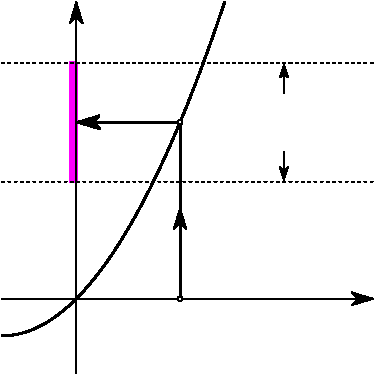
\includegraphics{figures/03epsAndNoDelta.pdf}}
    \put( -2.00,  92.85){\sffamily\itshape \makebox[0pt][r]{$L-\varepsilon$}}
    \put( -2.00, 149.81){\sffamily\itshape \makebox[0pt][r]{$L+\varepsilon$}}
    \put( 31.60, 121.33){\sffamily\itshape \makebox[0pt][r]{$L$}}
    \put(108.24, 168.50){\sffamily\itshape $y=f(x)$}
    \put( 84.44,  24.60){\sffamily\itshape $a$}
    \put( 91.44, 121.33){\sffamily\itshape \
How close must $x$ be to $a$ for $f(x)$ to end up in this range?
}
\end{picture}


  
\begin{picture} (180.000000,180.000000)(0,0)
\put(0.0, 0.0){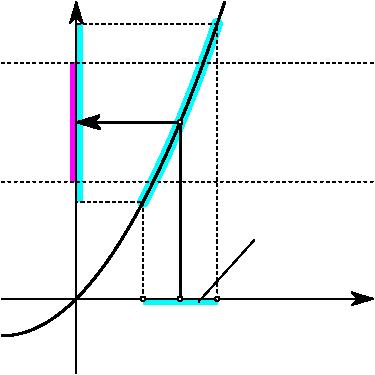
\includegraphics{figures/03epsAndDeltaTooBig.pdf}}
    \put( -2.00,  92.85){\sffamily\itshape \makebox[0pt][r]{$L-\varepsilon$}}
    \put( -2.00, 149.81){\sffamily\itshape \makebox[0pt][r]{$L+\varepsilon$}}
    \put( 31.60, 121.33){\sffamily\itshape \makebox[0pt][r]{$L$}}
    \put(108.24, 168.50){\sffamily\itshape $y=f(x)$}
    \put(107.24,  39.60){\sffamily\itshape $a+\delta$}
    \put( 44.64,  39.60){\sffamily\itshape $a-\delta$}
    \put( 84.44,  24.60){\sffamily\itshape $a$}
    \put(125.04,  64.72){\sffamily\itshape \begin{minipage}{240pt}
        For some $x$ in this interval $f(x)$ is not between
        $L-\varepsilon$ and $L+\varepsilon$. Therefore the $\delta$ in this
        picture is too big for the given $\varepsilon$.  You need a smaller
        $\delta$.
        \end{minipage}}
\end{picture}


  
\begin{picture} (180.000000,180.000000)(0,0)
\put(0.0, 0.0){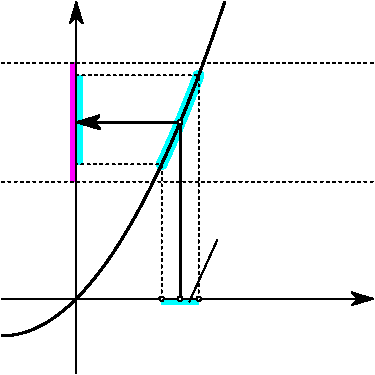
\includegraphics{figures/03epsAndDelta.pdf}}
    \put( -2.00,  92.85){\sffamily\itshape \makebox[0pt][r]{$L-\varepsilon$}}
    \put( -2.00, 149.81){\sffamily\itshape \makebox[0pt][r]{$L+\varepsilon$}}
    \put( 31.60, 121.33){\sffamily\itshape \makebox[0pt][r]{$L$}}
    \put(108.24, 168.50){\sffamily\itshape $y=f(x)$}
    \put( 98.34,  39.60){\sffamily\itshape $a+\delta$}
    \put( 53.54,  39.60){\sffamily\itshape $a-\delta$}
    \put( 84.44,  24.60){\sffamily\itshape $a$}
    \put(107.24,  64.72){\sffamily\itshape \begin{minipage}{240pt}
        If you choose $x$ in this interval then $f(x)$ will be between
        $L-\varepsilon$ and $L+\varepsilon$. Therefore the $\delta$ in this
        picture is small enough for the given $\varepsilon$.
        \end{minipage}}
\end{picture}

\end{figure}
When we first discussed the limit, say $\lim_{x \to 5} 2x + 1$, we made a table,
\begin{table}[H]
    \centering
    \begin{tabular}{|c|c|}
        \hline
        $x$ & $f(x) = 2x+1$ \\
        \hline
        5.1 & 11.2 \\
        5.01 & 11.02 \\
        5.001 & 11.002 \\
        4.9 & 10.8 \\
        4.99 & 10.98 \\
        4.999 & 10.998 \\
        \hline
    \end{tabular}
\end{table}
This table can be written also in this form.
\begin{table}[H]
    \centering
    \begin{tabular}{|c|c|}
        \hline
        $\abs{x-5}$ & $\abs{f(x)-11}$ \\
        \hline
        0.1 & 0.2 \\
        0.01 & 0.02 \\
        0.001 & 0.002 \\
        \hline
    \end{tabular}
\end{table}

It looks like for any $\epsilon>0$, if $\abs{x-5} < \frac{\epsilon}{2}$ then $\abs{f(x)-11}< \epsilon$. Now let's prove this!
\begin{example}
    Show that $\lim_{x\to5}2x+1=11$.
\end{example}
\begin{solution}
    We have $f(x) = 2x+1$, $a=5$ and $L=11$, and the question we must answer is
    ``how close should $x$ be to $5$ if you want to be sure that $f(x)=2x+1$
    differs less than $\epsilon$ from $L=11$?''

    \[
    |f(x)-L| = \abs{(2x+1)-11} = |2x-10| = 2\cdot |x-5| = 2\cdot |x-a|.
    \]
    So choose $\delta = \frac{\epsilon}{2}$. Then
    \[
    |f(x)-L|<\epsilon \text{ whenever } 0<|x-a|<\frac{\epsilon}{2}.
    \]
\end{solution}

\begin{example}[``Don't choose $\delta>1$'' trick]
    Show that $\lim_{x\to 3}x^2 = 9$.
\end{example}
\begin{solution}
    We have $f(x) = x^2$, $a=3$, $L=9$, and again the question is, ``how small
    should $|x-3|$ be to guarantee $|x^2-9|<\epsilon$?''

    \[
    |x^2-9| = |(x-3)(x+3)| = |x+3|\cdot|x-3|.
    \]
    Here is a trick that allows you to replace the factor $|x+3|$ with a
    constant.  We hereby agree \textit{that we always choose our $\delta$ so
    that $\delta\leq 1$.}  If we do that, then we will always have
    \[
    |x-3|<\delta\leq 1, \text{i.e. }|x-3|<1,
    \]
    or $2<x<4$ or $|x+1|<5$. Therefore
    \[
    |x^2-1| = |x+1|\cdot|x-1|<5|x-1|.
    \]
    So choose
    \[
    \delta = \min\{1, \frac{\epsilon}{5}\}.
    \]

    2nd way:
    Note that $|x+3|=|x-3+6|<|x-3|+6<\delta+6$
    \[
        \abs{f(x) - 9} = \abs{x+3}\abs{x-3} < (\delta+6) \delta
    \]
    So choose $(\delta+6) \delta < \epsilon$, or
    \[
        (\delta + 3)^2 < \epsilon + 9 \implies \delta < \sqrt{\epsilon + 9} - 3
    \]
\end{solution}

\begin{example}
    Show that $\lim_{x\to 4}1/x = 1/4$.
\end{example}
\begin{solution}
    We apply the definition with $a=4$, $L=1/4$ and $f(x) = 1/x$.
    Thus, for any $\epsilon>0$ we try to show that if $|x-4|$ is small
    enough then one has $|f(x)-1/4|<\epsilon$.

    We begin by estimating $|f(x)-\frac14|$ in terms of $|x-4|$:
    \[
    |f(x)-1/4| = \left|\frac1x-\frac14\right| = \left| \frac{4-x}{4x}\right| =
    \frac{|x-4|}{|4x|} =\frac{1}{|4x|}\,|x-4|.
    \]
    As before, things would be easier if $1/|4x|$ were a constant.  To achieve
    that we again agree not to take $\delta>1$.  If we always have $\delta\leq
    1$, then we will always have $|x-4|<1$, and hence $3<x<5$.  How large can
    $1/|4x|$ be in this situation?  Answer: the quantity $1/|4x|$ increases as
    you decrease $x$, so if $3<x<5$ then it will never be larger than
    $1/|4\cdot 3| = \frac1{12}$.

    We see that if we never choose $\delta>1$, we will always have
    \[
    |f(x) - \frac{1}{4}|\leq \frac{1}{12}|x-4| \quad\text{for}\quad |x-4|<\delta.
    \]
    To guarantee that $|f(x)-\frac14|<\epsilon$ we could threfore require
    \[
    \frac{1}{12} |x-4|<\epsilon, \quad\text{i.e.}\quad |x-4| <12\epsilon.
    \]
    Hence if we choose $\delta=12\epsilon$ or any smaller number, then
    $|x-4|<\delta$ implies $|f(x)-4|<\epsilon$.  Of course we have to honor
    our agreement never to choose $\delta>1$, so our choice of $\delta$ is
    \[
    \delta = \text{the smaller of }1\text{ and }12\epsilon = \min \bigl(1,
    12\epsilon\bigr).
    \]
\end{solution}

\begin{example}
    Verify that $\Lim{x}{2} \dfrac{x-2}{1+x^2} = 0$.
\end{example}
\begin{solution}
    Notice that $\dfrac{\abs{x-2}}{\abs{1+x^2}} < \abs{x-2}$ since $1+x^2 > 1$. Hence choose $\delta=\epsilon$.
\end{solution}

\end{document}